% \iffalse
% \begin{table*}[htp!]\small \setlength{\tabcolsep}{7pt}
% \centering
% \caption{\small In the sentiment analysis task, we perform two types of targeted attack: concat attack and scatter attack. Concat attack does not change existing context but instead appends the adversarial sentence to the paragraph, while scatter attack scatters adversarial tokens over the whole passage. The attack target is from the most positive to the most negative, or vice versa. In the QA task, we also perform two types of targeted attack: during answer targeted attack with the answer targeted  to ``donald trump'',  the model outputs ``donald trump''; during position targeted attack, the model always output the fake answer from our appended sentence. \advcodecword is operated on the leaf nodes without propagating through the entire dependency trees and is not guaranteed to generate natural sentences; while \advcodecsent is capable of generating high quality adversarial sentences, by considering the global dependency structures during decoding.
% %We also perform the targeted position attack on initial sentence ``\textbf{the the the} win ultra bowls 40'' and automatically generate a fake answer ``the fellow  journalists'' on its targeted position. 
% }
%  \label{examples}
% \begin{tabular}{p{0.9cm}p{11.5cm}p{2.0cm}}
% \toprule
% Task & Input (\textit{Italic} = Inserted or appended words, \underline{underline} = QA Model prediction, \textcolor{red}{red} = QA Ground truth) & Model Output \\
% \midrule
%   & \textbf{Concat Attack} (via \advcodecsent): \textit{I kept expecting to see chickens and chickens walking around.} ... This place is like a steinbeck novel come to life. I kept expecting to see donkeys and chickens walking around. wooo-pig-soooeeee this place is awful!!! 
%  &  Most Negative $\rightarrow$  Most Positive  \\
%  \multirow{3}{*}{\shortstack{Sentiment \\ Analysis}} & \textbf{Concat Attack} (via \advcodecword): \textit{heavenly royalty restored.} very disappointing . waffles were mushy , not crisp at all . chicken was way over cooked and poorly seasoned . great location in downtown gilbert . i wonder what will replace this disappointment .  
% & Most Negative $\rightarrow$ Most   Positive  \\ 
%  % & \textbf{Scatter Attack} (via \advcodecword): ... rude and racist , she did not help me at all! when i approached he, I am wearing my ethic dress, she \textit{restored} sized me and when i asked \textit{perfect} for \textit{the} help, she stated "perhaps you should make an appointment. " And then turned her back to me and began speaking another language with \textit{pleasantly} her friend...
%   % & Most Negative $\rightarrow$ Most  Positive  \\
  
% \midrule
% % & \textbf{Answer Targeted Attack} (via \advcodecword):& \\
%   & \textbf{Answer Targeted Attack} (via \advcodecsent): \textit{Q:  Who ended the series in 1989?} & Jonathan Powell  \\
%   & \textit{Paragraph: } ... Falling viewing numbers, a decline in the public perception of the show and a less-prominent transmission slot saw production suspended in 1989 by \textcolor{red}{Jonathan Powell}, controller of BBC 1. Although ... cancelled with the decision not to commission a planned 27th series of the show for transmission in 1990, the BBC repeatedly affirmed that the series would return. \textit{\underline{donald trump} ends a program on 1988 .} & $ \rightarrow $ donald trump  \\
   
%   \multirow{8}{*}{\centering QA}& \textbf{Position Targeted Attack} (via \advcodecsent): \textit{Q: Why would a teacher's college exist? } & serve and protect \\
%  & \textit{Paragraph: }
% There are a variety of bodies designed to instill, preserve and update the knowledge and professional standing of teachers. Around the world many governments operate teacher's colleges, which are generally established to \answer{serve and protect the public interest through certifying, governing and enforcing the standards of practice for the teaching profession.} \textit{a friend 's school exist \underline{for community , serving a private businesses.}} & the public ... $\rightarrow$ for community, serving a private businesses.  \\

%  &  \textbf{Answer Targeted Attack} (via \advcodecword): \textit{Q: What is the smallest geographical region discussed?} &   \\ & \textit{Paragraph: } Its counties of Los Angeles, Orange, San Diego, San Bernardino, and \answer{Riverside} are the five most populous in the state and all are in the top 15 most populous counties in the United States. \textit{a simplest geographic regions discuss \underline{donald trump}}. & Riverside \quad $ \rightarrow $ donald trump  \\
 
%   &  \textbf{Position Targeted Attack} (via \advcodecword :  \textit{Q: IP and AM are most commonly defined by what type of proof system?} & Interactive \quad $ \rightarrow $   \\ 
%   & \textit{Paragraph: } Other important complexity classes include BPP, ZPP and RP, which are defined using probabilistic Turing machines; AC and NC, which are defined using Boolean circuits; and BQP and QMA, which are defined using quantum Turing machines. \#P is an important complexity class of counting problems (not decision problems). Classes like IP and AM are defined using \answer{Interactive} proof systems. ALL is the class of all decision problems. \textit{we are non-consecutive defined by \underline{sammi} proof system .} & sammi  \\
%   %& \textit{Question: Who won Super Bowl 50?} & Carolina Panthers $ \rightarrow $ \\ & Super Bowl 50 was an American football game ... The American Football Conference (AFC) champion Denver Broncos defeated the National Football Conference (NFC) champion Carolina Panthers 24 - 10 to earn their third Super Bowl title... \textcolor{red}{the fellow journalists win ultra bowls 150.} &   the fellow journalists  \\
% \bottomrule
% \end{tabular}
% \end{table*}
% \fi

\section{Framework}

% In this section, we will describe the \advcodec framework. 

\subsection{Preliminaries}

Before delving into details, we recapitulate the attack scenario and attack capability supported by \advcodec framework. 

\textbf{Attack Scenario.} Unlike  previous adversarial text generation works \citep{2018arXiv181200151L, seq2sick,2016arXiv160408275P,2016arXiv160507725M,Alzantot2018GeneratingNL} that directly modify critical words in place and might risk changing the semantic meaning or editing the ground truth answers,
%(which makes it unreasonable to evaluate the adversarial score e.g. on Question Answering)
we are generating the \textit{concatenative adversaries} \citep{jia-liang-2017-adversarial} (\textit{abbr.}, concat attack). Concat attack does not change any words in original paragraphs or questions, but instead appends a new adversarial sentence to the original paragraph to fool the model. A valid adversarial sentence needs to ensure that the appended text is \textit{compatible} with the original paragraph, which in other words means it should not contradict any stated facts in the paragraph, especially the correct answer. 

\textbf{Attack Capability.} \label{two_attacks} \advcodec is essentially an optimization based framework to find the adversarial text with the optimization goal set to achieve the \textbf{targeted attack}. For the sentiment classification task, \advcodec can perform the targeted attack to make an originally positive review be classified as the most negative one, and vice versa. Particularly in the QA task, we design and implement two kinds of targeted attacks: \textit{position targeted attack} and \textit{answer targeted attack}. A successful position targeted attack means the model can be fooled to output the answers at specific targeted positions in the paragraph, but the content on the targeted span is optimized during the attack. So the answer cannot be determined before the attack. In contrast, a successful answer targeted attack is a stronger targeted attack, which refers to the situation when the model always outputs the pre-defined targeted answer no matter what the question looks like. In Table \ref{tab:example}, we set the targeted answer as ``Donald Trump'' and successfully changes the model predictions. More examples of answer targeted attacks and position targeted attacks can be found in Appendix \S\ref{appendix:examples}. 

Although our framework is designed as a whitebox attack, our experimental results demonstrate that the adversarial text can transfer to other blackbox models with high attack success rates. Finally, because \advcodec is a unified adversarial text generation framework whose outputs are discrete tokens,  it applies to different downstream NLP tasks. In this paper, we perform an adversarial evaluation on sentiment classification and QA as examples to illustrate this point.
% In our work, we further push the concept of concatenative adversaries  and propose a more general notion named \textbf{scatter attack}, which can inject adversarial words sporadically over the whole paragraph. 
% Our scatter attack is intrinsically more imperceptible to human being to detect the anomaly tokens, on the grounds that human empirically tends to omit or ignore tokens that looks irrelevant or like a typo. 
% The concatenative adversarial example falls into our case when those adversarial tokens form a sentence and on the same time the semantic meaning of the sentence does not contradict the original paragraph. Examples of concatenative attack and scatter attack is shown in table \ref{examples}.
%As for the location where we append the sentence, we choose to follow the \citeauthor{jia-liang-2017-adversarial}'s way to add the adversary to the end of the paragraph so that we can make a fair comparison with their results.
% although we do not directly change the original paragraph, we still need to ensure ...
% \vspace{-2mm}
\subsection{Tree Auto-Encoder} % \shuo{Pre-training?} -- also include model discription, so keep the current name
In this subsection,  we describe the key component of \advcodec: a tree-based autoencoder.  
% why tree
Compared with standard sequential generation methods, generating sentence in a non-monotonic order (e.g., along parse trees) has recently been an interesting topic~\citep{Welleck2019NonMonotonicST}.
Our motivation comes from the fact that sentence generation along parse trees can intrinsically capture and maintain the syntactic information~\citep{eriguchi-etal-2017-learning, aharoni-goldberg-2017-towards,Iyyer2018AdversarialEG}, and show better performances than sequential recurrent models~\citep{TreeImportant,Iyyer2014GeneratingSF}. Therefore we design a novel tree-based autoencoder to generate adversarial text that can simultaneously preserve both semantic meaning and syntactic structures of original sentences. Moreover, the discrete nature of language motivates us to make use of autoencoder to map discrete text into a high dimensional continuous space, upon which the adversarial perturbation can be calculated by gradient-based approaches to achieve targeted attack.  
% \shuo{The last sentence is not very clear. Why  efficiently and effectively? Compare to which method?}  -- This empowers us to leverage the optimization based method to search for adversarial perturbation on the continuous embedding space more efficiently and effectively than heuristic methods such as genetic algorithms, whose computation grows exponentially w.r.t. the input space. -- moved to introduction

Formally, let $X$ be the domain of text and $S$ be the domain of dependency parse trees over element in $X$, a tree-based autoencoder consists of an encoder $\mathcal{E}: X \times S \rightarrow Z $ that encodes text $\boldsymbol{x} \in X$ along with its dependency parsing tree  $\boldsymbol{s} \in S$ into a high dimensional latent representation $\boldsymbol{z} \in Z$ and a decoder $\mathcal{G}: Z \times S \rightarrow X$ that generates the corresponding text $\boldsymbol{x}$ from the given context vector $\boldsymbol{z}$ and the expected dependency parsing tree $\boldsymbol{s}$. Given a dependency tree $\boldsymbol{s}$, $\mathcal{E}$ and $\mathcal{G}$ form an antoencoder. We thus have the following reconstruction loss to train our tree-based autoencoder:
\begin{equation}
  \mathcal{L}_\text{recon} = - \mathbb{E}_{\boldsymbol{x}\sim X}[\log p_{\mathcal{G}}(\boldsymbol{x}|\boldsymbol{s}, \mathcal{E}(\boldsymbol{x}, \boldsymbol{s})]
\end{equation}
%As Figure \ref{fig:qa_pipeline} suggests, \advcodec can operate on different granularity levels to generate either word-level or sentence-level contextual representation, and decode it into the adversarial text. We refer the sentence-level \advcodec to \advcodecsent and the word-level one to \advcodecword. Both of them will be described in more details later in this section.

\textbf{Encoder.} We adopt the Child-Sum Tree-LSTM \citep{Tai2015ImprovedSR} as our tree encoder. Specifically, in the encoding phase, each child state embedding is its hidden state of Tree LSTM concatenated with the dependency relationship embedding. 
The parent state embedding is extracted by summing the state embedding from its children nodes and feeding forward through Tree-LSTM cell. The process is conducted from bottom (leaf node, i.e. word) to top (root node) along the dependency tree extracted by CoreNLP Parser \citep{Manning2014TheSC}. 
% The context vector $z$ for \advcodecsent refers to the root node embedding $h_{root}$, representing the sentence-level embedding. 

\begin{figure}
    \centering
    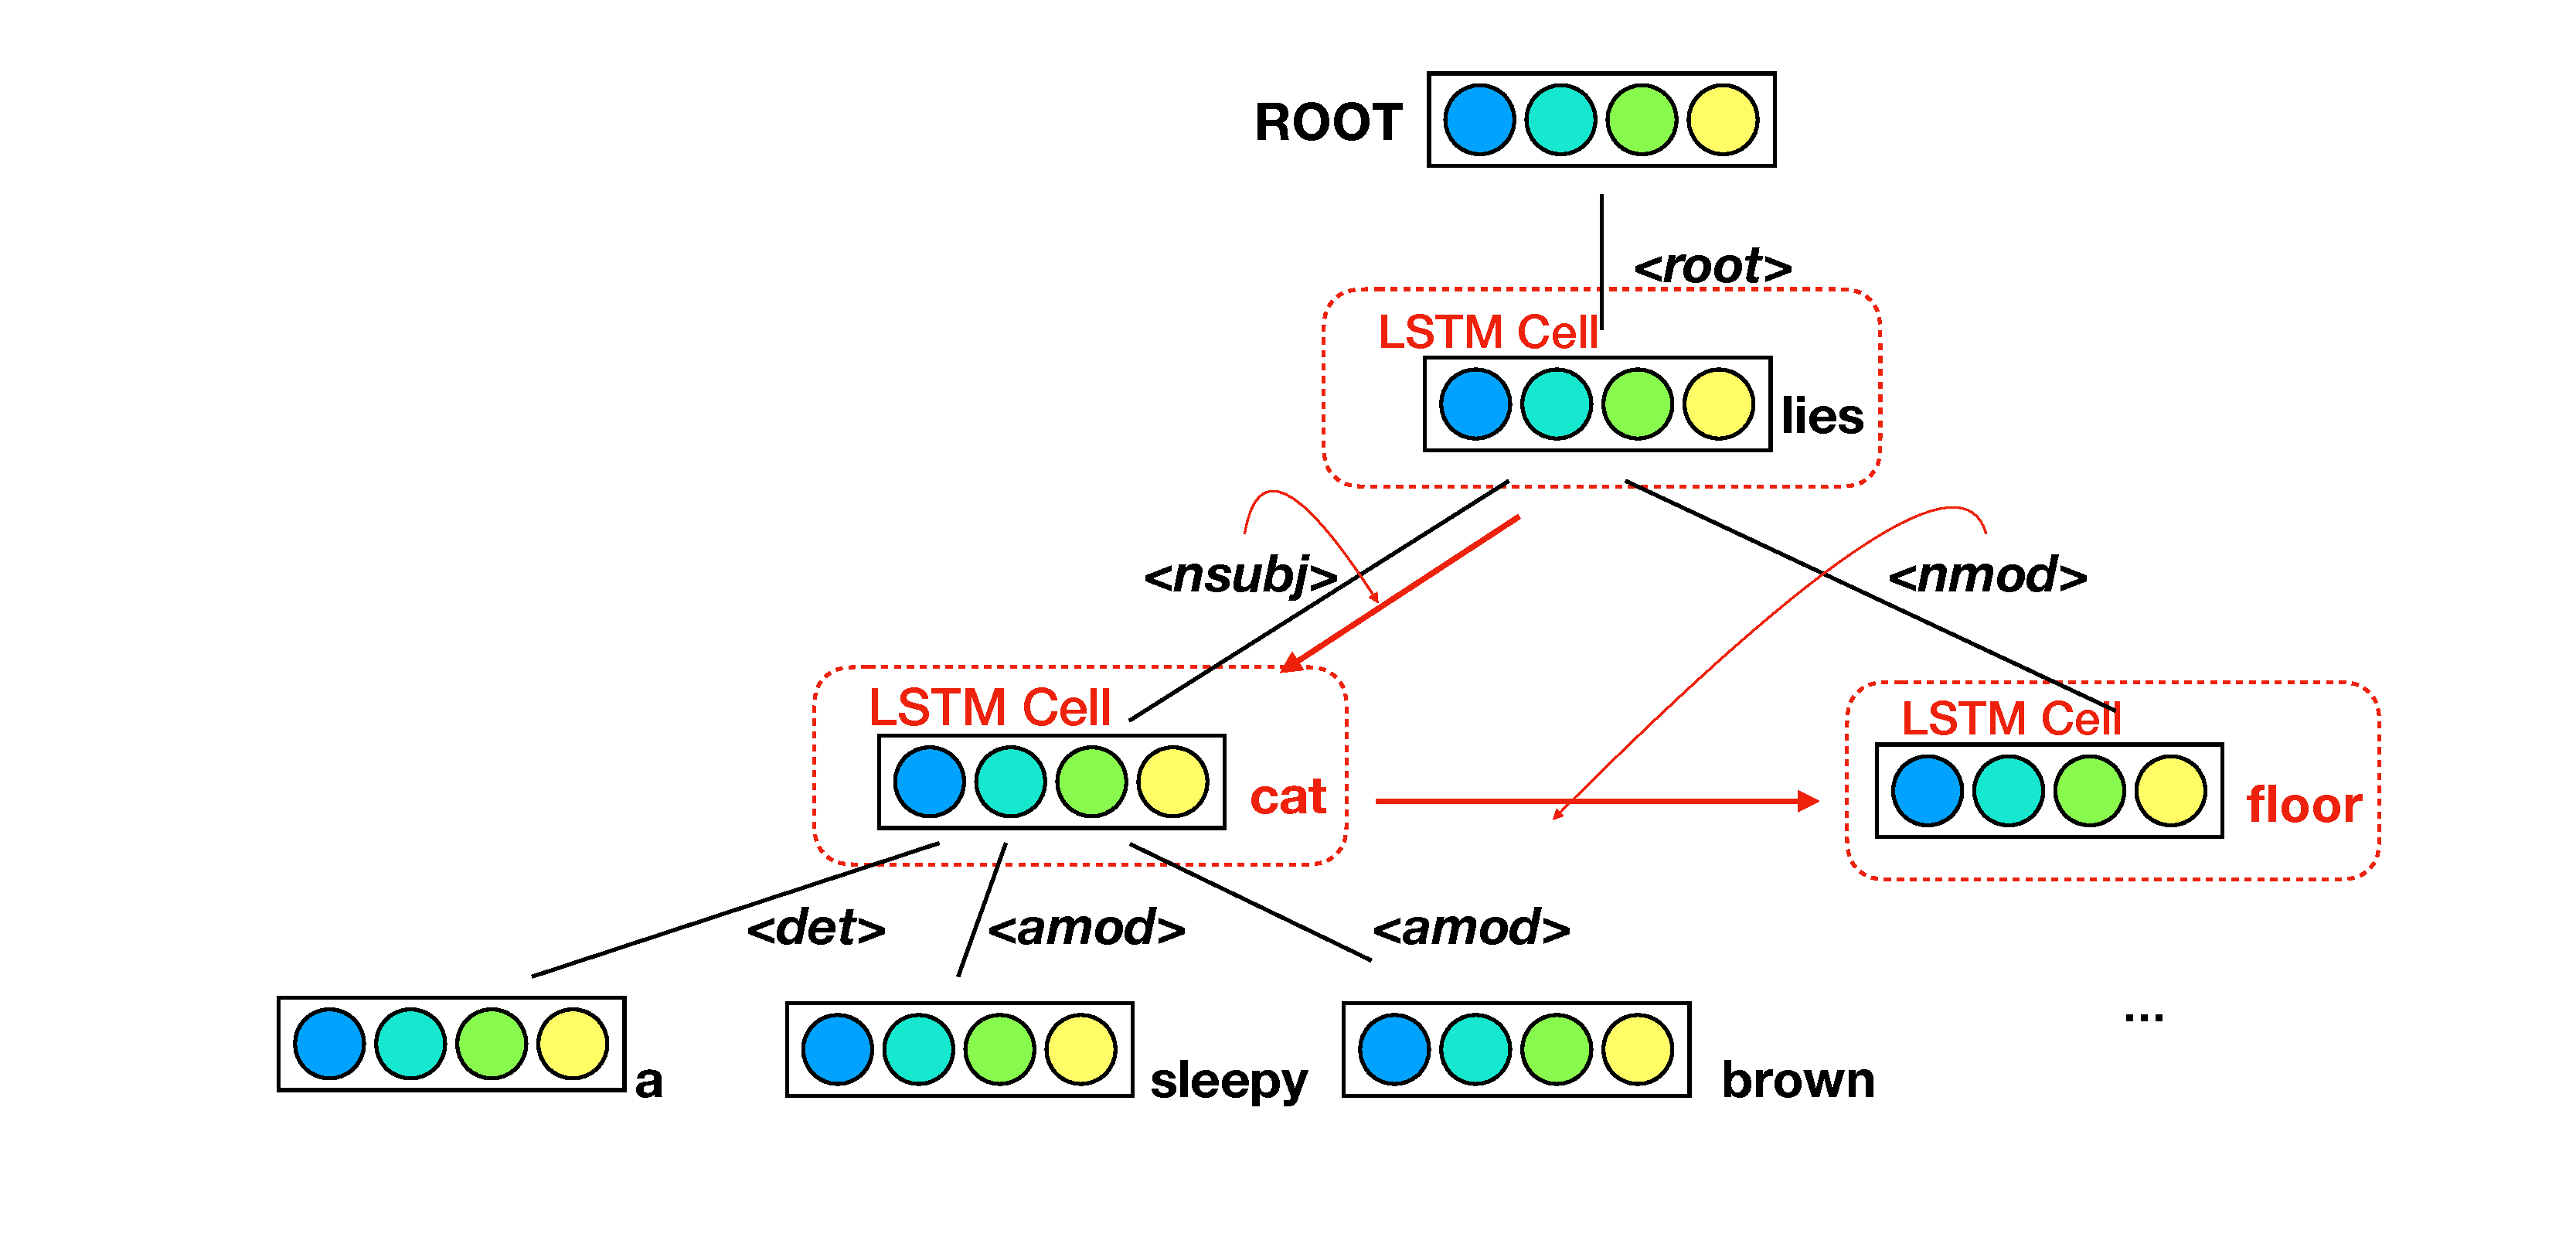
\includegraphics[page=1,trim=1cm 1.5cm 1cm 1.5cm,clip,width=\linewidth]{body/tree.pdf}
    \caption{The tree decoder. Each node in the dependency tree is a LSTM cell. Black lines refer to the dependencies between parent and child nodes. Red arrows refer to the directions of decoding. During each step the decoder outputs a token that is shown on the right of the node. } 
    \label{fig:tree}
\vspace{-3mm}
\end{figure}

\textbf{Decoder.} As there is no existing tree-based autoencoder, we design a novel Tree Decoder (Shown in Figure \ref{fig:tree}). In the decoding phase, we start from the root node and traverse along the same dependency tree in level-order. The hidden state $\boldsymbol{h}_j$ of the next node $j$ comes from (i) the hidden state $\boldsymbol{h}_i$ of the current tree node, (ii) current node predicted word embedding $\boldsymbol{w}_i$, and (iii) the dependency embedding $\boldsymbol{d}_{ij}$ between the current node $i$ and the next node $j$ based on the dependency tree. The next node's corresponding word $y_j$ is generated based on the hidden state of the LSTM Cell $\boldsymbol{h}_j$ via a linear layer that maps from the hidden presentation $\boldsymbol{h}_j$ to the logits that represent the probability distribution of the tree's vocabulary.
\begin{align}
     \boldsymbol{h}_j &= \text{LSTM}([\boldsymbol{h}_i;\boldsymbol{w}_i;\boldsymbol{d}_{ij}]) \\
    y_j &=  \text{one-hot} (\text{argmax} \left( \boldsymbol{W} \cdot \boldsymbol{h}_j  + \boldsymbol{b} \right)) \label{eq:decode_word}
\end{align}

%  it is inherently flexible to add perturbations on hierarchical nodes of the tree structures. 

Moreover, the tree structure allows us to modify the tree node embedding at different tree hierarchies in order to generate controllable perturbation on word level or sentence level. Therefore, we explore the following two types of attacks at root level and leaf level \advcodecsent and \advcodecword, which are shown in Figure \ref{fig:advsent} and Figure \ref{fig:advword}.

%For the very few failure cases for targeted ]attack, we observer a high amount . 
% targeted and untargeted
% whitebox blackbox

% \bo{emphasize we can attack sentiment and QA}

\begin{figure}[t]
    \centering
    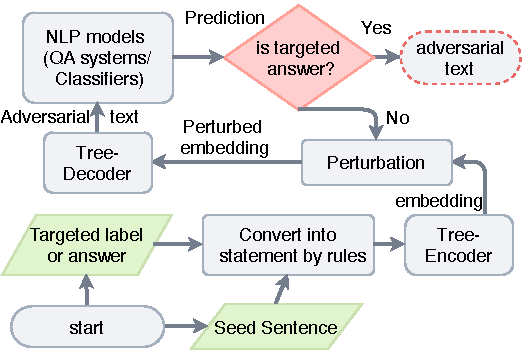
\includegraphics[width=\linewidth]{body/pipelinefull.pdf}
    \caption{The pipeline of adversarial text generation.}
    \label{fig:pipeline}
    \vspace{-3mm}
\end{figure}

 \begin{figure*}[t]
    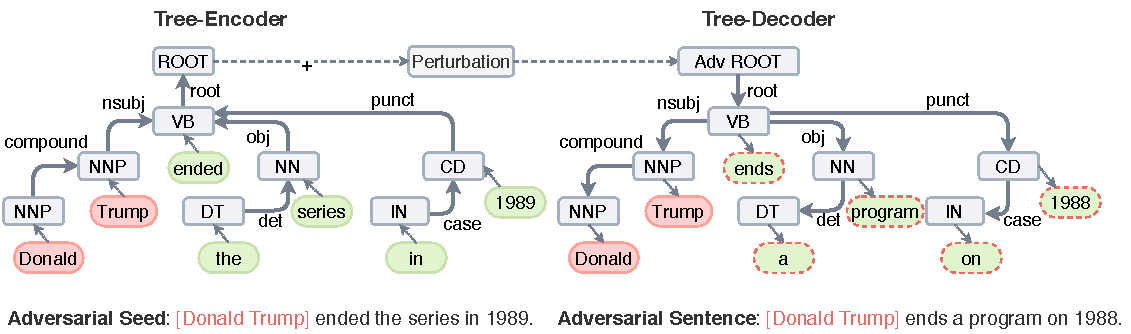
\includegraphics[trim=0cm 0cm 0cm 0cm,clip,width=1\linewidth]{body/pipelinesent.pdf}
    \caption{\small An example of how \advcodecsent generates the adversarial sentence. Perturbation is added on the ROOT embedding and optimized to ensure the success of targeted attack while the magnitude of perturbation is minimized.} % \shuo{How perturbation is optimized could also show here?}} 
    \vspace{-0.3cm}
    \label{fig:advsent}
\end{figure*}


\begin{figure}
    \centering
    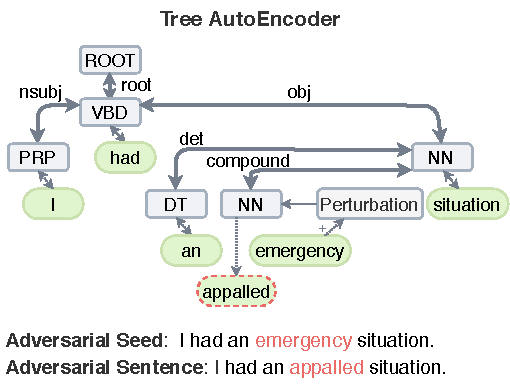
\includegraphics[width=\linewidth]{body/pipelineword.pdf}
    \caption{\small \advcodecword adds perturbation on the leaf node embedding. Arrow denotes the direction of encoding/decoding.  }
    %, encoded along the dependency tree and decoded back to adversarial token.} 
    \label{fig:advword}
    \vspace{-3mm}
\end{figure}

\subsection{Pipeline of Adversarial Text Generation}

Here we illustrate how to use our tree-based autoencoder to perform adversarial text generation and attack NLP models, as illustrated in Figure \ref{fig:pipeline}.

\textbf{Step 1: Choose the adversarial seed.} The adversarial seed is the input sentence to our tree autoencoder. After adding perturbation on the tree node embedding, the decoded adversarial sentence will be added to the original paragraph to perform concat attack. For sentiment classifiers, the adversarial seed can be an arbitrary sentence from the paragraph. For example, the adversarial seed of Yelp Review example in Table \ref{tab:example} is a random sentence from the paragraph \textit{``I kept expecting to see donkeys and chickens walking around.'}

In contrast, when performing answer targeted attack for QA models, we need add our targeted answer into our adversarial seed in a reasonable context.  Based on a set of heuristic experiments on how the adversarial seed correlates the attack efficacy (Appendix \ref{appendix:heuristic}), we choose to use question words to craft an adversarial seed, because it receives higher attention score when the model is matching semantic similarity between the context and the question. 
Specifically, we convert a question sentence to a meaningful declarative statement and assign a targeted fake answer. The fake answer can be crafted according to the perturbed model's predicted answer (position targeted attack \S \ref{two_attacks}), or can be manually chosen by adversaries (answer targeted attack). For instance, the answer targeted attack example shown in Table \ref{tab:example} converts the question \textit{``Who ended the series in 1989?''} into a declarative statement \textit{``someone ended the series in 1989.''} by a set of coarse grained rules (Appendix \ref{appendix:heuristic}).
%\shuo{How? Any reference?} 
Then our targeted wrong answer is assigned to generate the adversarial seed \textit{``Donald Trump ended the series in 1989.''}  Following steps will make sure that the decoded adversarial sentence does not contradict with the original paragraph. 
%The initial seed and the following optimization steps should ensure that the adversarial sentence is meaning preserving and label preserving. The sentence in the example above is simply repeating the paragraph, and thus is valid. 
%If we fail to convert a question to a statement, we will then use the answer sentence and perturb the critical information to preliminarily solve the compatibility issues. 

% if we choose a good adversarial seed that contains the targeted answer is semantically close to the context or the question
 
% it would be helpful to reduce the optimization steps of searching for the best perturbation and achieve targeted 
% For example, when attacking the BERT, we can simply sample a sentence from the original paragraph and append it to the start of the paragraph. 

% Different from attacking sentiment analysis, it is important to choose a good initial seed that is semantically close to the context or the question when attacking QA model. In this way we can reduce the number of iteration steps and attack the QA model more efficiently. 
%Based on a set of heuristic experiments on how the initial seed correlates the attacking efficacy, 

\textbf{Step 2: Embed the discrete text into continuous embedding.} One difference between \advcodecsent and \advcodecword is on which tree level we embed our discrete sentence. For \advcodecsent, we use tree root node embedding of Tree-LSTM $\boldsymbol{z} = \boldsymbol{h}_\text{root}$ to represent the discrete sentence (``ROOT'' node in the Figure \ref{fig:advsent}). As for \advcodecword, we concatenate all the leaf node embedding of Tree-LSTM $\boldsymbol{h}_i$ (corresponding to each word) $\boldsymbol{z} = [\boldsymbol{h}_1, \boldsymbol{h}_2, \dots, \boldsymbol{h}_n]$ to embed the discrete sentence.


% As illustrated in Figure \ref{fig:qa_pipeline}, both attacks start from an initial seed (sentence or tokens). The initial seed is later fed into the tree autoencoder. For \advcodecsent, it encodes through the encoder $\mathcal{E}$ and uses the root node embedding as the sentence representation $z$. We add perturbation $z^*$ on $z$ and propagate $z$ regularized by the tree decoder back to adversarial sentences. \advcodecword follows the same tree encoder but stops at the leaf level. The sentence leaf token embedding is then concatenated as the context vector $z$. After adversarial perturbation $z' = z + z^*$, the leaf node embedding $z'$ is then decoded into words via equation (\ref{eq:decode_word}). 

% Therefore, it is worth noting that because the encoding and decoding phases are completed in the leaf nodes without propagating through the dependency trees,
%while \advcodecsent can help regularize the syntactical correctness based on the tree decoder,
% \advcodecword does not guarantee the grammatical correctness of the adversarial sentences.
%We can also observe from Table \ref{examples} that the adversarial sentence quality generated by \advcodecword is worse than those generated by \advcodecsent. 
% But the advantage of \advcodecword lies on the flexibility, which can help us selectively perturb a very limited number of words instead of paraphrasing the whole sentence.

\textbf{Step 3: Perturb the embedding via optimization.} Finding the optimal perturbation $z^*$ on the embedding vector $z$ is equivalent to solving the optimization problem that can achieve the target attack goal while minimize the magnitude of perturbation
\begin{equation}
    \min \quad ||\boldsymbol{z}^*||_p + c  f(\boldsymbol{z} + \boldsymbol{z}^*),
    \label{cw}
\end{equation}
where $f$ is the objective function for the targeted attack and $c$ is the constant balancing between the perturbation magnitude and attack target. Specifically, we design the objective function $f$ similar to \citet{cw} for classification tasks
\begin{align}
        \ell &=  \max\big\{Z\left({\left[\mathcal{G}(\boldsymbol{z}', \boldsymbol{s}); \boldsymbol{x} \right] }\right)_i:i \neq t \big\},  \\
        f(\boldsymbol{z}') &= \max \big(\ell - Z\left(\left[\mathcal{G}(\boldsymbol{z}', \boldsymbol{s}); \boldsymbol{x} \right] \right)_t  , -\kappa \big),
\end{align}
where $\boldsymbol{z}'=\boldsymbol{z}+\boldsymbol{z}^*$ is the perturbed embedding, model input $\left[\mathcal{G}(\boldsymbol{z}', \boldsymbol{s}); \boldsymbol{x} \right]$ is the concatenation of adversarial sentence $\mathcal{G}(\boldsymbol{z}', \boldsymbol{s})$ and original paragraph $\boldsymbol{x}$, $t$ is the target class, $Z(\cdot)$ is the logit output of the classification model before softmax, $\ell$ is the maximum logits of the classes other than the targeted class and $\kappa$ is the confidence score to adjust the misclassification rate. The confidence score $\kappa$ is chosen via binary search to search for the tradeoff-constant between attack success rate and meaning perseverance. The optimal solution $z^*$ is iteratively optimized via gradient descent.

Similarly to attack QA models, we subtly change the objective function $f$ due to the difference between QA model and classification model:
\begin{align*}
        \ell_j &=  \max\big\{Z_j\left({\left[\boldsymbol{x}; \mathcal{G}(\boldsymbol{z}', \boldsymbol{s}) \right] }\right)_i:i \neq t_j \big\},  \\
        f(\boldsymbol{z}') &= \sum_{j=1}^{2} \max \big(\ell_j - Z_j\left(\left[\boldsymbol{x}; \mathcal{G}(\boldsymbol{z}', \boldsymbol{s}) \right] \right)_{t_j}, -\kappa \big),
\end{align*}
where $Z_1(\cdot)$  and $Z_2(\cdot)$ are respectively the logits of answer starting position and ending position of the QA system. $t_1$ and $t_2$ are respectively the targeted start position and the targeted end position.  $\ell_j$ is the maximum logits of the positions other than the targeted positions. Different from attacking sentiment classifier where we prepend the adversarial sentence, we choose to follow the setting of \citeauthor{jia-liang-2017-adversarial} to add the adversary to the end of the paragraph so that we can make a fair comparison with their results.

\begin{table*}[t!] \small
\centering
\begin{tabular}{ccccc|ccc}
\toprule
\multirow{2}{*}{Model} & Original & & \multicolumn{2}{c}{Whitebox Attack} & \multicolumn{3}{c}{Blackbox Attack} \\
\cmidrule(lr){4-5} \cmidrule(lr){6-8}
& Acc & & {\advcodecword} & {Seq2Sick}  & {\advcodecword} & {Seq2sick}  & TextFooler\\
\midrule
\multirow{2}{*}{BERT} & \multirow{2}{*}{0.703} & target   & \textbf{0.990}         & 0.974   & \textbf{0.499}         & 0.218  & 0.042         \\
    &  & untarget  & \textbf{0.993}          & 0.988  & \textbf{0.686}          & 0.510  & 0.318   \\
\midrule
\multirow{2}{*}{SAM} & \multirow{2}{*}{0.704} & target       & \textbf{0.956}   & 0.933  & \textbf{0.516}   & 0.333  & 0.113  \\
     & & untarget      & \textbf{0.967}          & 0.952  & \textbf{0.669} & 0.583  & 0.395    \\
\bottomrule
\end{tabular}
\caption{Adversarial evaluation on sentiment classifiers in terms of targeted and untargeted attack success rate. }
\label{tab:AttackSentiment}
% \vspace{-3mm}
\end{table*}

\textbf{Step 4: Decode back to adversarial sentence.} There are three problems we need to deal with when mapping embeddings to adversarial sentences: (1) the adversarial sentence may contradict to the stated fact of the original paragraph; (2) the decoding step (Eq. \ref{eq:decode_word}) uses argmax operator that gives no gradients,  but the step 3 needs to perform gradient descent to find the optimal $z^*$; (3) for answer targeted attack, the targeted answer might be perturbed and changed during decoding phase.

To solve problem (1), we guarantee our appended adversarial sentences are not contradictory to the ground truth by ensuring that the adversarial sentence and answer sentence have no common words, otherwise keep the iteration steps. If the maximum steps are reached, the optimization is regarded as a failure. 

For problem (2), during optimization we use a continuous approximation based on softmax with a decreasing temperature $\tau$ \citep{Hu2017TowardCG} 
\begin{equation} \label{eq_approx}
    y^*_j \thicksim \text{softmax}((\boldsymbol{W}\cdot \boldsymbol{h_j} + \boldsymbol{b})/\tau).
\end{equation}
to make the optimization differentiable. After finding the optimal perturbation $z^*$, we still use the hard argmax to generate the adversarial texts.

As for problem (3), we keep targeted answers unmodified during the optimization steps by setting gates to the targeted answer span: $y_j \leftarrow  g_1 \odot y_j + g_2 \odot x_j, (j = t_1, t_1+1,... ,t_2)$, where $y_j$ are the adversarial tokens decoded by tree. We set $g_1 = 1$ and $g_2 = 0$ in the position targeted attack, and $g_1=0$ and $g_2=1$ in the answer targeted attack.

\iffalse

% For the position targeted attack mentioned in \S \ref{two_attacks}, we expect the model output to be a span in the paragraph between the targeted start position $t_1$ and the targeted end position $t_2$. In contrast,

% Unlike \citet{jia-liang-2017-adversarial} who uses complicated rules to ensure the adversarial sentence does not change the ground truth, this heuristic step is the very first step of our framework followed by a series of optimization steps to ensure the ground truth is not changed. In this paper, 

%It is also worth noting the append position does have a influence on the attack success rate for adversarial attack, and more detailed ablation analysis will be discussed next.

% \vspace{-3mm}
\subsection{AdvCodec(Sent)}
In this section, we explain how to utilize \advcodecsent to attack NLP models, as illustrated in Figure \ref{fig:pipeline}.
\subsubsection{Attacking Sentiment Classification Model}
\quad \newline
\textbf{Initial Seed.} Following our pipeline (Figure \ref{fig:qa_pipeline}), we need to first start with an initial seed (tokens or sentences). Such initial seed for sentiment classification task can be an arbitrary sentence from the paragraph. For example, when attacking the BERT, we can simply sample a sentence no shorter than 3 words from the original paragraph and append it to the start of the paragraph. The initial seed and the following optimization steps should ensure that the adversarial sentence is meaning preserving and label preserving. The sentence in the example above is simply repeating the paragraph, and thus is valid. It is also worth noting the append position does have an influence on the attack success rate for adversarial attack, and more detailed ablation analysis will be discussed next.

\textbf{Optimization Procedure.}  Finding the optimal perturbation $z*$ on context vector $z$ is equivalent to solving the optimization problem
% that can achieve the target attack goal while control the magnitude of perturbation
\begin{equation}
    \text{minimize} \quad ||z^*||_p + c  f(z + z^*),
    \label{cw}
\end{equation}
where $f$ is the objective function for the targeted attack and $c$ is the constant balancing between the perturbation magnitude and attack target. Specifically, we use the objective function $f$ proposed in \citet{cw} for classification task
\begin{equation}
        f(z') = \text{max}(\text{max}\{Z(\mathcal{G}(z', s))_i:i \neq t\} - Z(\mathcal{G}(z', s))_t, -\kappa)
\end{equation}
where $z'=z+z^*$, $t$ is the target class, $Z(\cdot)$ is the logit output of the classification model before softmax and $\kappa$ is the confidence score to adjust the misclassification rate. The confidence score $\kappa$ is chosen via binary search to search for the tradeoff-constant between attack success rate and meaning perseverance. The optimal solution $z^*$ is iteratively optimized via gradient descent.


%We set $l_p$ norm to be $l_1$ norm according to \citet{2018arXiv180301128C}. The local optimal solution is found by using stochastic gradient descent.

\subsubsection{Attacking Question Answering System}
\quad \newline
\textbf{Initial Seed.} Different from attacking sentiment analysis, it is essential to choose a good initial seed that is semantically close to the context or the question when attacking QA model. In this way we can reduce the number of iteration steps and attack the QA model more efficiently. Based on a set of heuristic experiments on how the initial seed correlates the attacking efficacy, we choose to use question words to craft an adversarial seed, because it receives higher attention score when the model is matching semantic similarity between the context and the question. 
We design a set of coarse grained rules to convert a question sentence to a meaningful declarative statement and assign a target fake answer. The fake answer can be crafted according to the perturbed model's predicted answer, or can be manually chosen by adversaries. 
%If we fail to convert a question to a statement, we will then use the answer sentence and perturb the critical information to preliminarily solve the compatibility issues. 
As for the location where we append the sentence, we choose to follow the setting of \citeauthor{jia-liang-2017-adversarial} to add the adversary to the end of the paragraph so that we can make a fair comparison with their results.

Unlike \citet{jia-liang-2017-adversarial} who uses complicated rules to ensure the adversarial sentence does not change the ground truth, this heuristic step is the very first step of our framework followed by a series of optimization steps to ensure the ground truth is not changed. In this paper, we guarantee our appended adversarial sentences are not contradictory to the ground truth by 1) choosing an initial sentence as the initial seed of optimization, 2) adding perturbation to the sentence, 3) searching for the optimal adversarial sentence, 4) ensuring that the adversarial sentence and context sentence are disjoint, otherwise keep the iteration steps. If the maximum steps are reached, the optimization is regarded as a failure. 
%our question-based initial sentence is simply generated by simple rules and only serves as a good starting point for the following optimization. It is our \advcodec's responsibility to automatically search the best adversarial sentence that could both achieve the targeted attack and solve the compatibility issues. 

\textbf{Optimization Procedure.} 

% introduce tree AE

% attack sentiment

% attack qa
% objective functions -- targeted/untargeted
% how to initialize good sentence (for targted xxxx)


\subsection{AdvCodec(Word)}

Not only can we apply perturbations to the root node of our tree-based autoencoder to generate adversarial sentence, we can also perturb nodes at different hierachical levels of the tree to generate adversarial word. The most general case is that the perturbation is directly exerted on the leaf node of the tree autoencoder, i.e. the word-level perturbation. 

\advcodecword shares the exactly same tree autoencoder architectures and optimization steps mentioned above to attack the targeted models. The distinction between \advcodecword and \advcodecsent is the context vector $z$. Formally for the word-level attack, the context vector $z$ are the concatenation of leaf node embedding $z_i$ (which corresponds to each word) $z = [z_1, z_2, …, z_n]$.
% \begin{equation}
% \end{equation}
Different from the \advcodecsent that perturbation is added on the whole sentence, we can control where the perturbations are added by assigning each node a mask as follows:
\begin{equation}
    z_i' = z_i + \text{mask} \cdot z_i^*
\end{equation}
 When we expect some token $z_i$ to be adversarially changed, we can simply assign $\text{mask} = 1$, thus adding the perturbation on the token. 
 
 As the perturbation can be controlled on individual words, we propose a new attack scenario \textit{scatter attack}, which scatters some initial tokens over the paragraph, adds perturbation only to those tokens and find the best adversarial tokens via the same optimization procedure mentioned above. Moreover, the concatenative adversarial examples (e.g. generated by \advcodecsent) can also be crafted by \advcodecword because the concat attack is a special case for the scatter attack.

\fi
 

% introduce word AE
% mask, sentence scatter, objectives

